\documentclass{book}
\usepackage[a4paper,top=2.5cm,bottom=2.5cm,left=2.5cm,right=2.5cm]{geometry}
\usepackage{makeidx}
\usepackage{natbib}
\usepackage{graphicx}
\usepackage{multicol}
\usepackage{float}
\usepackage{listings}
\usepackage{color}
\usepackage{ifthen}
\usepackage[table]{xcolor}
\usepackage{textcomp}
\usepackage{alltt}
\usepackage{ifpdf}
\ifpdf
\usepackage[pdftex,
            pagebackref=true,
            colorlinks=true,
            linkcolor=blue,
            unicode
           ]{hyperref}
\else
\usepackage[ps2pdf,
            pagebackref=true,
            colorlinks=true,
            linkcolor=blue,
            unicode
           ]{hyperref}
\usepackage{pspicture}
\fi
\usepackage[utf8]{inputenc}
\usepackage{mathptmx}
\usepackage[scaled=.90]{helvet}
\usepackage{courier}
\usepackage{sectsty}
\usepackage[titles]{tocloft}
\usepackage{doxygen}
\lstset{language=C++,inputencoding=utf8,basicstyle=\footnotesize,breaklines=true,breakatwhitespace=true,tabsize=8,numbers=left }
\makeindex
\setcounter{tocdepth}{3}
\renewcommand{\footrulewidth}{0.4pt}
\renewcommand{\familydefault}{\sfdefault}
\hfuzz=15pt
\setlength{\emergencystretch}{15pt}
\hbadness=750
\tolerance=750
\begin{document}
\hypersetup{pageanchor=false,citecolor=blue}
\begin{titlepage}
\vspace*{7cm}
\begin{center}
{\Large Xsiliumserver }\\
\vspace*{1cm}
{\large Generated by Doxygen 1.8.0}\\
\vspace*{0.5cm}
{\small Sat Mar 3 2012 23:03:12}\\
\end{center}
\end{titlepage}
\clearemptydoublepage
\pagenumbering{roman}
\tableofcontents
\clearemptydoublepage
\pagenumbering{arabic}
\hypersetup{pageanchor=true,citecolor=blue}
\chapter{Class Index}
\section{Class Hierarchy}
This inheritance list is sorted roughly, but not completely, alphabetically\-:\begin{DoxyCompactList}
\item \contentsline{section}{A\-U\-T\-H\-\_\-\-L\-O\-G\-O\-N\-\_\-\-C\-H\-A\-L\-L\-E\-N\-G\-E\-\_\-\-C}{\pageref{struct_a_u_t_h___l_o_g_o_n___c_h_a_l_l_e_n_g_e___c}}{}
\item \contentsline{section}{A\-U\-T\-H\-\_\-\-L\-O\-G\-O\-N\-\_\-\-P\-R\-O\-O\-F\-\_\-\-C}{\pageref{struct_a_u_t_h___l_o_g_o_n___p_r_o_o_f___c}}{}
\item \contentsline{section}{A\-U\-T\-H\-\_\-\-L\-O\-G\-O\-N\-\_\-\-P\-R\-O\-O\-F\-\_\-\-S}{\pageref{struct_a_u_t_h___l_o_g_o_n___p_r_o_o_f___s}}{}
\item \contentsline{section}{Authentification}{\pageref{class_authentification}}{}
\item \contentsline{section}{auth\-Server}{\pageref{classauth_server}}{}
\item \contentsline{section}{Postgre\-S\-Q\-L\-Interface}{\pageref{class_postgre_s_q_l_interface}}{}
\begin{DoxyCompactList}
\item \contentsline{section}{Login\-Database}{\pageref{class_login_database}}{}
\end{DoxyCompactList}
\item \contentsline{section}{s\-Client}{\pageref{structs_client}}{}
\item \contentsline{section}{Signal\-Exception}{\pageref{class_signal_exception}}{}
\item \contentsline{section}{Signal\-Handler}{\pageref{class_signal_handler}}{}
\end{DoxyCompactList}

\chapter{Class Index}
\section{Class List}
Here are the classes, structs, unions and interfaces with brief descriptions\-:\begin{DoxyCompactList}
\item\contentsline{section}{\hyperlink{struct_a_u_t_h___l_o_g_o_n___c_h_a_l_l_e_n_g_e___c}{A\-U\-T\-H\-\_\-\-L\-O\-G\-O\-N\-\_\-\-C\-H\-A\-L\-L\-E\-N\-G\-E\-\_\-\-C} }{\pageref{struct_a_u_t_h___l_o_g_o_n___c_h_a_l_l_e_n_g_e___c}}{}
\item\contentsline{section}{\hyperlink{struct_a_u_t_h___l_o_g_o_n___p_r_o_o_f___c}{A\-U\-T\-H\-\_\-\-L\-O\-G\-O\-N\-\_\-\-P\-R\-O\-O\-F\-\_\-\-C} }{\pageref{struct_a_u_t_h___l_o_g_o_n___p_r_o_o_f___c}}{}
\item\contentsline{section}{\hyperlink{struct_a_u_t_h___l_o_g_o_n___p_r_o_o_f___s}{A\-U\-T\-H\-\_\-\-L\-O\-G\-O\-N\-\_\-\-P\-R\-O\-O\-F\-\_\-\-S} }{\pageref{struct_a_u_t_h___l_o_g_o_n___p_r_o_o_f___s}}{}
\item\contentsline{section}{\hyperlink{class_authentification}{Authentification} }{\pageref{class_authentification}}{}
\item\contentsline{section}{\hyperlink{classauth_server}{auth\-Server} }{\pageref{classauth_server}}{}
\item\contentsline{section}{\hyperlink{class_login_database}{Login\-Database} }{\pageref{class_login_database}}{}
\item\contentsline{section}{\hyperlink{class_postgre_s_q_l_interface}{Postgre\-S\-Q\-L\-Interface} }{\pageref{class_postgre_s_q_l_interface}}{}
\item\contentsline{section}{\hyperlink{structs_client}{s\-Client} }{\pageref{structs_client}}{}
\item\contentsline{section}{\hyperlink{class_signal_exception}{Signal\-Exception} }{\pageref{class_signal_exception}}{}
\item\contentsline{section}{\hyperlink{class_signal_handler}{Signal\-Handler} }{\pageref{class_signal_handler}}{}
\end{DoxyCompactList}

\chapter{Class Documentation}
\hypertarget{struct_a_u_t_h___l_o_g_o_n___c_h_a_l_l_e_n_g_e___c}{\section{A\-U\-T\-H\-\_\-\-L\-O\-G\-O\-N\-\_\-\-C\-H\-A\-L\-L\-E\-N\-G\-E\-\_\-\-C Struct Reference}
\label{struct_a_u_t_h___l_o_g_o_n___c_h_a_l_l_e_n_g_e___c}\index{A\-U\-T\-H\-\_\-\-L\-O\-G\-O\-N\-\_\-\-C\-H\-A\-L\-L\-E\-N\-G\-E\-\_\-\-C@{A\-U\-T\-H\-\_\-\-L\-O\-G\-O\-N\-\_\-\-C\-H\-A\-L\-L\-E\-N\-G\-E\-\_\-\-C}}
}
\subsection*{Public Attributes}
\begin{DoxyCompactItemize}
\item 
\hypertarget{struct_a_u_t_h___l_o_g_o_n___c_h_a_l_l_e_n_g_e___c_aeae61a22cd55f7c638252be18eb60b30}{uint8\-\_\-t {\bfseries cmd}}\label{struct_a_u_t_h___l_o_g_o_n___c_h_a_l_l_e_n_g_e___c_aeae61a22cd55f7c638252be18eb60b30}

\item 
\hypertarget{struct_a_u_t_h___l_o_g_o_n___c_h_a_l_l_e_n_g_e___c_a9940a1075f1f87d6a1c0ea66276e07d0}{uint8\-\_\-t {\bfseries error}}\label{struct_a_u_t_h___l_o_g_o_n___c_h_a_l_l_e_n_g_e___c_a9940a1075f1f87d6a1c0ea66276e07d0}

\item 
\hypertarget{struct_a_u_t_h___l_o_g_o_n___c_h_a_l_l_e_n_g_e___c_a1f8350f5e288085f6f8b02edbe5066d5}{uint16\-\_\-t {\bfseries size}}\label{struct_a_u_t_h___l_o_g_o_n___c_h_a_l_l_e_n_g_e___c_a1f8350f5e288085f6f8b02edbe5066d5}

\item 
\hypertarget{struct_a_u_t_h___l_o_g_o_n___c_h_a_l_l_e_n_g_e___c_afe16cdd01959b8359007898ed9fe4eaf}{uint8\-\_\-t {\bfseries version1}}\label{struct_a_u_t_h___l_o_g_o_n___c_h_a_l_l_e_n_g_e___c_afe16cdd01959b8359007898ed9fe4eaf}

\item 
\hypertarget{struct_a_u_t_h___l_o_g_o_n___c_h_a_l_l_e_n_g_e___c_a4adc97b95b3e27fd31c156305d7a6d2f}{uint16\-\_\-t {\bfseries build}}\label{struct_a_u_t_h___l_o_g_o_n___c_h_a_l_l_e_n_g_e___c_a4adc97b95b3e27fd31c156305d7a6d2f}

\item 
\hypertarget{struct_a_u_t_h___l_o_g_o_n___c_h_a_l_l_e_n_g_e___c_a75c0962888103ce2f59fb25d9eacddad}{uint8\-\_\-t {\bfseries platform} \mbox{[}4\mbox{]}}\label{struct_a_u_t_h___l_o_g_o_n___c_h_a_l_l_e_n_g_e___c_a75c0962888103ce2f59fb25d9eacddad}

\item 
\hypertarget{struct_a_u_t_h___l_o_g_o_n___c_h_a_l_l_e_n_g_e___c_ab1a2af6201b54dcab4f7b486acbc2318}{uint8\-\_\-t {\bfseries os} \mbox{[}4\mbox{]}}\label{struct_a_u_t_h___l_o_g_o_n___c_h_a_l_l_e_n_g_e___c_ab1a2af6201b54dcab4f7b486acbc2318}

\item 
\hypertarget{struct_a_u_t_h___l_o_g_o_n___c_h_a_l_l_e_n_g_e___c_a01a5a5f1f6871196ef14b46b01b00ce2}{uint8\-\_\-t {\bfseries country} \mbox{[}4\mbox{]}}\label{struct_a_u_t_h___l_o_g_o_n___c_h_a_l_l_e_n_g_e___c_a01a5a5f1f6871196ef14b46b01b00ce2}

\item 
\hypertarget{struct_a_u_t_h___l_o_g_o_n___c_h_a_l_l_e_n_g_e___c_ae3e396f841fba34f270aee2ebfa8a8b0}{uint32\-\_\-t {\bfseries timezone\-\_\-bias}}\label{struct_a_u_t_h___l_o_g_o_n___c_h_a_l_l_e_n_g_e___c_ae3e396f841fba34f270aee2ebfa8a8b0}

\item 
\hypertarget{struct_a_u_t_h___l_o_g_o_n___c_h_a_l_l_e_n_g_e___c_ad395212aa21e73ccd09ad1c8c89d56b3}{uint8\-\_\-t {\bfseries login\-\_\-len}}\label{struct_a_u_t_h___l_o_g_o_n___c_h_a_l_l_e_n_g_e___c_ad395212aa21e73ccd09ad1c8c89d56b3}

\item 
\hypertarget{struct_a_u_t_h___l_o_g_o_n___c_h_a_l_l_e_n_g_e___c_a7927c7d748c63f13e57784dc162b2932}{uint8\-\_\-t {\bfseries login} \mbox{[}1\mbox{]}}\label{struct_a_u_t_h___l_o_g_o_n___c_h_a_l_l_e_n_g_e___c_a7927c7d748c63f13e57784dc162b2932}

\end{DoxyCompactItemize}


The documentation for this struct was generated from the following file\-:\begin{DoxyCompactItemize}
\item 
src/server/\-Shared/\-Structure/Client.\-h\end{DoxyCompactItemize}

\hypertarget{struct_a_u_t_h___l_o_g_o_n___p_r_o_o_f___c}{\section{A\-U\-T\-H\-\_\-\-L\-O\-G\-O\-N\-\_\-\-P\-R\-O\-O\-F\-\_\-\-C Struct Reference}
\label{struct_a_u_t_h___l_o_g_o_n___p_r_o_o_f___c}\index{A\-U\-T\-H\-\_\-\-L\-O\-G\-O\-N\-\_\-\-P\-R\-O\-O\-F\-\_\-\-C@{A\-U\-T\-H\-\_\-\-L\-O\-G\-O\-N\-\_\-\-P\-R\-O\-O\-F\-\_\-\-C}}
}
\subsection*{Public Attributes}
\begin{DoxyCompactItemize}
\item 
\hypertarget{struct_a_u_t_h___l_o_g_o_n___p_r_o_o_f___c_ab5ebb6c258f8c8145dde05d6f51676ca}{int {\bfseries cmd}}\label{struct_a_u_t_h___l_o_g_o_n___p_r_o_o_f___c_ab5ebb6c258f8c8145dde05d6f51676ca}

\item 
\hypertarget{struct_a_u_t_h___l_o_g_o_n___p_r_o_o_f___c_a0b6e6d937878d6899fb0a9edcfb2a855}{int {\bfseries A} \mbox{[}32\mbox{]}}\label{struct_a_u_t_h___l_o_g_o_n___p_r_o_o_f___c_a0b6e6d937878d6899fb0a9edcfb2a855}

\item 
\hypertarget{struct_a_u_t_h___l_o_g_o_n___p_r_o_o_f___c_a22532519abfd579165db2411eec927cc}{int {\bfseries M1} \mbox{[}20\mbox{]}}\label{struct_a_u_t_h___l_o_g_o_n___p_r_o_o_f___c_a22532519abfd579165db2411eec927cc}

\item 
\hypertarget{struct_a_u_t_h___l_o_g_o_n___p_r_o_o_f___c_ac2503bd2e46a810e9a1b8b49bcb63116}{int {\bfseries crc\-\_\-hash} \mbox{[}20\mbox{]}}\label{struct_a_u_t_h___l_o_g_o_n___p_r_o_o_f___c_ac2503bd2e46a810e9a1b8b49bcb63116}

\item 
\hypertarget{struct_a_u_t_h___l_o_g_o_n___p_r_o_o_f___c_a383f7c9cee71121e3591c988e41f6ccf}{int {\bfseries number\-\_\-of\-\_\-keys}}\label{struct_a_u_t_h___l_o_g_o_n___p_r_o_o_f___c_a383f7c9cee71121e3591c988e41f6ccf}

\item 
\hypertarget{struct_a_u_t_h___l_o_g_o_n___p_r_o_o_f___c_af99249ee0b3a4987fff8f910c5f70ef7}{int {\bfseries security\-Flags}}\label{struct_a_u_t_h___l_o_g_o_n___p_r_o_o_f___c_af99249ee0b3a4987fff8f910c5f70ef7}

\end{DoxyCompactItemize}


The documentation for this struct was generated from the following file\-:\begin{DoxyCompactItemize}
\item 
src/server/\-Shared/\-Structure/Client.\-h\end{DoxyCompactItemize}

\hypertarget{struct_a_u_t_h___l_o_g_o_n___p_r_o_o_f___s}{\section{A\-U\-T\-H\-\_\-\-L\-O\-G\-O\-N\-\_\-\-P\-R\-O\-O\-F\-\_\-\-S Struct Reference}
\label{struct_a_u_t_h___l_o_g_o_n___p_r_o_o_f___s}\index{A\-U\-T\-H\-\_\-\-L\-O\-G\-O\-N\-\_\-\-P\-R\-O\-O\-F\-\_\-\-S@{A\-U\-T\-H\-\_\-\-L\-O\-G\-O\-N\-\_\-\-P\-R\-O\-O\-F\-\_\-\-S}}
}
\subsection*{Public Attributes}
\begin{DoxyCompactItemize}
\item 
\hypertarget{struct_a_u_t_h___l_o_g_o_n___p_r_o_o_f___s_a30828bf0578791a8b330490a409716b0}{int {\bfseries cmd}}\label{struct_a_u_t_h___l_o_g_o_n___p_r_o_o_f___s_a30828bf0578791a8b330490a409716b0}

\item 
\hypertarget{struct_a_u_t_h___l_o_g_o_n___p_r_o_o_f___s_a28ceb2a20906e022ac88b185a3ebac41}{int {\bfseries error}}\label{struct_a_u_t_h___l_o_g_o_n___p_r_o_o_f___s_a28ceb2a20906e022ac88b185a3ebac41}

\item 
\hypertarget{struct_a_u_t_h___l_o_g_o_n___p_r_o_o_f___s_a0f5a8b365ae22988210d4e70ef102581}{int {\bfseries M2} \mbox{[}20\mbox{]}}\label{struct_a_u_t_h___l_o_g_o_n___p_r_o_o_f___s_a0f5a8b365ae22988210d4e70ef102581}

\end{DoxyCompactItemize}


The documentation for this struct was generated from the following file\-:\begin{DoxyCompactItemize}
\item 
src/server/\-Shared/\-Structure/Server.\-h\end{DoxyCompactItemize}

\hypertarget{class_authentification}{\section{Authentification Class Reference}
\label{class_authentification}\index{Authentification@{Authentification}}
}
\subsection*{Public Member Functions}
\begin{DoxyCompactItemize}
\item 
\hypertarget{class_authentification_a9cc153ac26a7a5e4c0dd56c2182ef7aa}{bool {\bfseries Create\-Client} (Packet $\ast$packet)}\label{class_authentification_a9cc153ac26a7a5e4c0dd56c2182ef7aa}

\item 
\hypertarget{class_authentification_a6734ee2fa780263443592cc2f02d918a}{bool {\bfseries Delete\-Client} (Packet $\ast$packet)}\label{class_authentification_a6734ee2fa780263443592cc2f02d918a}

\item 
\hypertarget{class_authentification_af1808489bd4c2e74507c549d5466f582}{bool {\bfseries Find\-Client} (Rak\-Net\-G\-U\-I\-D guid)}\label{class_authentification_af1808489bd4c2e74507c549d5466f582}

\item 
\hypertarget{class_authentification_ae1e5a8942e31c667d05ff94fd64e1236}{bool {\bfseries \-\_\-\-Handle\-Logon\-Challenge} (Rak\-Net\-::\-Packet $\ast$packet)}\label{class_authentification_ae1e5a8942e31c667d05ff94fd64e1236}

\item 
\hypertarget{class_authentification_a4749f3ed73e17a79a7e74a7f162fda49}{bool {\bfseries \-\_\-\-Handle\-Logon\-Proof} ()}\label{class_authentification_a4749f3ed73e17a79a7e74a7f162fda49}

\item 
\hypertarget{class_authentification_a409cdd1e3d0ce83c8834571918c6011d}{bool {\bfseries \-\_\-\-Handle\-Reconnect\-Challenge} ()}\label{class_authentification_a409cdd1e3d0ce83c8834571918c6011d}

\item 
\hypertarget{class_authentification_adfc637be23b0cf114e201b6275d71264}{bool {\bfseries \-\_\-\-Handle\-Reconnect\-Proof} ()}\label{class_authentification_adfc637be23b0cf114e201b6275d71264}

\item 
\hypertarget{class_authentification_a097485114d8bd1e9c36cd0c6b4a38a4a}{bool {\bfseries \-\_\-\-Handle\-Realm\-List} ()}\label{class_authentification_a097485114d8bd1e9c36cd0c6b4a38a4a}

\end{DoxyCompactItemize}


The documentation for this class was generated from the following files\-:\begin{DoxyCompactItemize}
\item 
src/server/\-Auth/\-Authentification/Authentification.\-h\item 
src/server/\-Auth/\-Authentification/Authentification.\-cpp\end{DoxyCompactItemize}

\hypertarget{classauth_server}{\section{auth\-Server Class Reference}
\label{classauth_server}\index{auth\-Server@{auth\-Server}}
}
\subsection*{Public Member Functions}
\begin{DoxyCompactItemize}
\item 
\hypertarget{classauth_server_ac406ba141a6f86f0f5bffe5542492188}{void {\bfseries start\-Thread} ()}\label{classauth_server_ac406ba141a6f86f0f5bffe5542492188}

\item 
\hypertarget{classauth_server_a4b76b1c2e6422d27671b7ea3e59d8910}{void {\bfseries stop\-Thread} ()}\label{classauth_server_a4b76b1c2e6422d27671b7ea3e59d8910}

\end{DoxyCompactItemize}


The documentation for this class was generated from the following files\-:\begin{DoxyCompactItemize}
\item 
src/server/\-Auth/Auth\-Server.\-h\item 
src/server/\-Auth/Auth\-Server.\-cpp\end{DoxyCompactItemize}

\hypertarget{class_login_database}{\section{Login\-Database Class Reference}
\label{class_login_database}\index{Login\-Database@{Login\-Database}}
}
Inheritance diagram for Login\-Database\-:\begin{figure}[H]
\begin{center}
\leavevmode
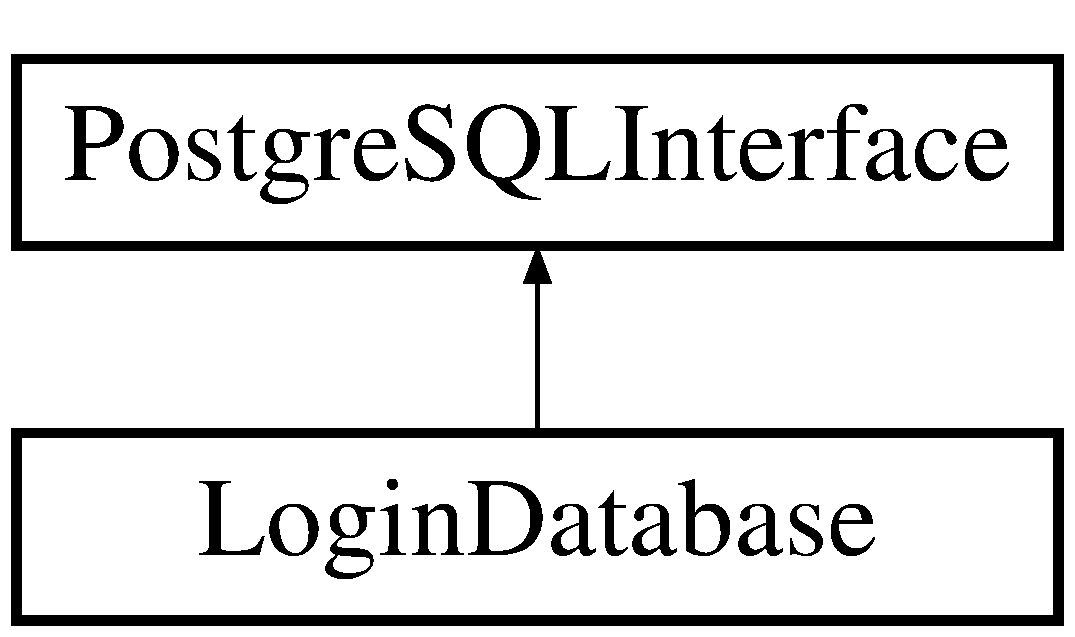
\includegraphics[height=2.000000cm]{class_login_database}
\end{center}
\end{figure}
\subsection*{Public Member Functions}
\begin{DoxyCompactItemize}
\item 
\hypertarget{class_login_database_a74087482da1d24ad9696d8d01567b060}{bool {\bfseries select\-Account} (const char $\ast$user\-Name, \hyperlink{structs_client}{s\-Client} $\ast$client)}\label{class_login_database_a74087482da1d24ad9696d8d01567b060}

\item 
\hypertarget{class_login_database_a5f832944039f157abb45cb1fe466e9e9}{bool {\bfseries get\-I\-P\-Ban} (std\-::string $\ast$I\-P, bool $\ast$results)}\label{class_login_database_a5f832944039f157abb45cb1fe466e9e9}

\item 
\hypertarget{class_login_database_af107de3014fcced25a111490455d76d5}{bool {\bfseries set\-I\-P\-Ban} ()}\label{class_login_database_af107de3014fcced25a111490455d76d5}

\end{DoxyCompactItemize}


The documentation for this class was generated from the following files\-:\begin{DoxyCompactItemize}
\item 
src/server/\-Shared/\-Databases/Login\-Database.\-h\item 
src/server/\-Shared/\-Databases/Login\-Database.\-cpp\end{DoxyCompactItemize}

\hypertarget{class_postgre_s_q_l_interface}{\section{Postgre\-S\-Q\-L\-Interface Class Reference}
\label{class_postgre_s_q_l_interface}\index{Postgre\-S\-Q\-L\-Interface@{Postgre\-S\-Q\-L\-Interface}}
}
Inheritance diagram for Postgre\-S\-Q\-L\-Interface\-:\begin{figure}[H]
\begin{center}
\leavevmode
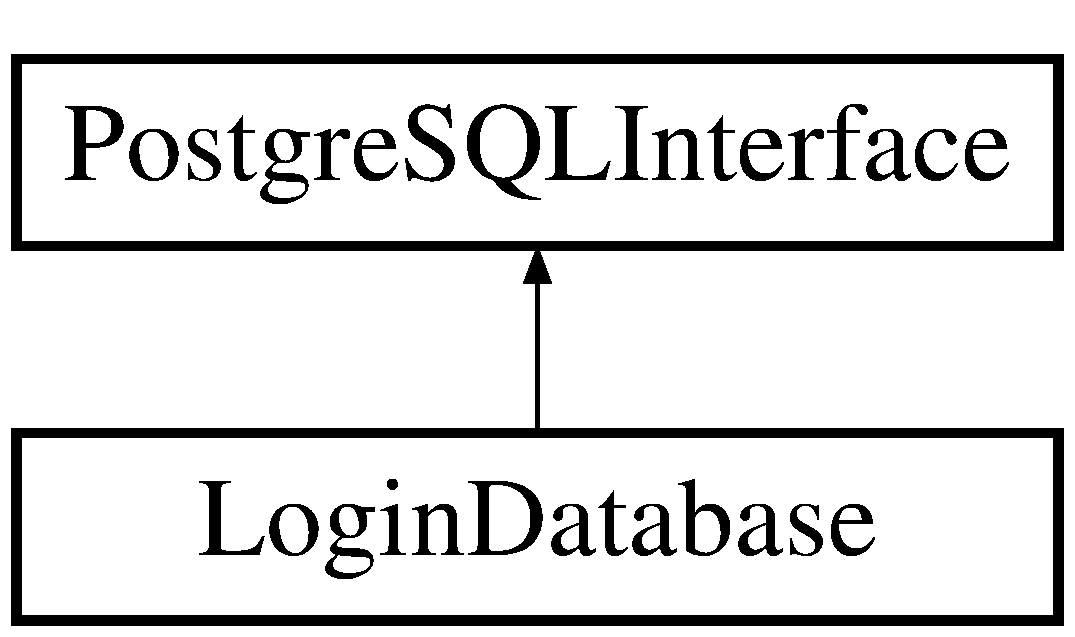
\includegraphics[height=2.000000cm]{class_postgre_s_q_l_interface}
\end{center}
\end{figure}
\subsection*{Public Member Functions}
\begin{DoxyCompactItemize}
\item 
bool \hyperlink{class_postgre_s_q_l_interface_a76c4ebdbd06ee57a4c69e5778c362724}{Connect} (const char $\ast$conninfo)
\item 
\hypertarget{class_postgre_s_q_l_interface_a761568edccdc320383683da86c5dfe7e}{void \hyperlink{class_postgre_s_q_l_interface_a761568edccdc320383683da86c5dfe7e}{Assign\-Connection} (P\-Gconn $\ast$\-\_\-pg\-Conn)}\label{class_postgre_s_q_l_interface_a761568edccdc320383683da86c5dfe7e}

\begin{DoxyCompactList}\small\item\em Use a connection allocated elsewehre. \end{DoxyCompactList}\item 
\hypertarget{class_postgre_s_q_l_interface_ad8a87839a70b64902f78063211e2e769}{P\-Gconn $\ast$ \hyperlink{class_postgre_s_q_l_interface_ad8a87839a70b64902f78063211e2e769}{Get\-P\-G\-Conn} (void) const }\label{class_postgre_s_q_l_interface_ad8a87839a70b64902f78063211e2e769}

\begin{DoxyCompactList}\small\item\em Get the instance of P\-Gconn. \end{DoxyCompactList}\item 
\hypertarget{class_postgre_s_q_l_interface_a62e68986cdc1e9eb2f308bdc135570ca}{void \hyperlink{class_postgre_s_q_l_interface_a62e68986cdc1e9eb2f308bdc135570ca}{Disconnect} (void)}\label{class_postgre_s_q_l_interface_a62e68986cdc1e9eb2f308bdc135570ca}

\begin{DoxyCompactList}\small\item\em Disconnect from the database. \end{DoxyCompactList}\item 
\hypertarget{class_postgre_s_q_l_interface_a6ecf3b86569fd0cdbc995b2ad0a6ee2b}{virtual const char $\ast$ \hyperlink{class_postgre_s_q_l_interface_a6ecf3b86569fd0cdbc995b2ad0a6ee2b}{Get\-Last\-Error} (void) const }\label{class_postgre_s_q_l_interface_a6ecf3b86569fd0cdbc995b2ad0a6ee2b}

\begin{DoxyCompactList}\small\item\em If any of the above functions fail, the error string is stored internally. Call this to get it. \end{DoxyCompactList}\item 
\hypertarget{class_postgre_s_q_l_interface_a7e0d635dd6f48c173568c738d9a5f10e}{long long {\bfseries Get\-Epoch} (void)}\label{class_postgre_s_q_l_interface_a7e0d635dd6f48c173568c738d9a5f10e}

\item 
\hypertarget{class_postgre_s_q_l_interface_a50903829c1ca03cada78ba3432cbcdc9}{char $\ast$ {\bfseries Get\-Local\-Timestamp} (void)}\label{class_postgre_s_q_l_interface_a50903829c1ca03cada78ba3432cbcdc9}

\item 
\hypertarget{class_postgre_s_q_l_interface_a64221c9df6cbe51daedebbe84771973b}{P\-Gresult $\ast$ {\bfseries Query\-Variadic} (const char $\ast$input,...)}\label{class_postgre_s_q_l_interface_a64221c9df6cbe51daedebbe84771973b}

\item 
\hypertarget{class_postgre_s_q_l_interface_ab62653db173f9d87b5e69fc0f5de4cb9}{bool {\bfseries Execute\-Blocking\-Command} (const char $\ast$command, P\-Gresult $\ast$$\ast$result, bool rollback\-On\-Failure)}\label{class_postgre_s_q_l_interface_ab62653db173f9d87b5e69fc0f5de4cb9}

\item 
\hypertarget{class_postgre_s_q_l_interface_a08e84ef50b92e38e038c9579ed83bedb}{bool {\bfseries Is\-Result\-Successful} (P\-Gresult $\ast$result, bool rollback\-On\-Failure)}\label{class_postgre_s_q_l_interface_a08e84ef50b92e38e038c9579ed83bedb}

\item 
\hypertarget{class_postgre_s_q_l_interface_addd65c7a8120fe778706086bf875c4c4}{void {\bfseries Rollback} (void)}\label{class_postgre_s_q_l_interface_addd65c7a8120fe778706086bf875c4c4}

\item 
\hypertarget{class_postgre_s_q_l_interface_a230ee730d970e7b4b41351e1cea4407e}{Rak\-Net\-::\-Rak\-String {\bfseries Get\-Escaped\-String} (const char $\ast$input) const }\label{class_postgre_s_q_l_interface_a230ee730d970e7b4b41351e1cea4407e}

\end{DoxyCompactItemize}
\subsection*{Static Public Member Functions}
\begin{DoxyCompactItemize}
\item 
\hypertarget{class_postgre_s_q_l_interface_aa3364b9afb4acf6e5d3fc3a25d06094c}{static bool {\bfseries P\-Q\-Get\-Value\-From\-Binary} (int $\ast$output, P\-Gresult $\ast$result, unsigned int row\-Index, const char $\ast$column\-Name)}\label{class_postgre_s_q_l_interface_aa3364b9afb4acf6e5d3fc3a25d06094c}

\item 
\hypertarget{class_postgre_s_q_l_interface_a85cbefe8d04c7b73ce17013965c43077}{static bool {\bfseries P\-Q\-Get\-Value\-From\-Binary} (int $\ast$output, P\-Gresult $\ast$result, int row\-Index, const char $\ast$column\-Name)}\label{class_postgre_s_q_l_interface_a85cbefe8d04c7b73ce17013965c43077}

\item 
\hypertarget{class_postgre_s_q_l_interface_a856e8b1615b1b1462cb8984a82663861}{static bool {\bfseries P\-Q\-Get\-Value\-From\-Binary} (unsigned int $\ast$output, P\-Gresult $\ast$result, int row\-Index, const char $\ast$column\-Name)}\label{class_postgre_s_q_l_interface_a856e8b1615b1b1462cb8984a82663861}

\item 
\hypertarget{class_postgre_s_q_l_interface_a2a78c3d71b28f7eb0332b566a9105d15}{static bool {\bfseries P\-Q\-Get\-Value\-From\-Binary} (long long $\ast$output, P\-Gresult $\ast$result, int row\-Index, const char $\ast$column\-Name)}\label{class_postgre_s_q_l_interface_a2a78c3d71b28f7eb0332b566a9105d15}

\item 
\hypertarget{class_postgre_s_q_l_interface_a961de63e792b5161141c8c3f30b0e635}{static bool {\bfseries P\-Q\-Get\-Value\-From\-Binary} (float $\ast$output, P\-Gresult $\ast$result, int row\-Index, const char $\ast$column\-Name)}\label{class_postgre_s_q_l_interface_a961de63e792b5161141c8c3f30b0e635}

\item 
\hypertarget{class_postgre_s_q_l_interface_a5293404d7c822fa3aacf7708852939b7}{static bool {\bfseries P\-Q\-Get\-Value\-From\-Binary} (double $\ast$output, P\-Gresult $\ast$result, int row\-Index, const char $\ast$column\-Name)}\label{class_postgre_s_q_l_interface_a5293404d7c822fa3aacf7708852939b7}

\item 
\hypertarget{class_postgre_s_q_l_interface_a5d5016039feff442d532391867dd0750}{static bool {\bfseries P\-Q\-Get\-Value\-From\-Binary} (bool $\ast$output, P\-Gresult $\ast$result, int row\-Index, const char $\ast$column\-Name)}\label{class_postgre_s_q_l_interface_a5d5016039feff442d532391867dd0750}

\item 
\hypertarget{class_postgre_s_q_l_interface_af6d32518de06bdd6371c05360d33e598}{static bool {\bfseries P\-Q\-Get\-Value\-From\-Binary} (Rak\-Net\-::\-Rak\-String $\ast$output, P\-Gresult $\ast$result, int row\-Index, const char $\ast$column\-Name)}\label{class_postgre_s_q_l_interface_af6d32518de06bdd6371c05360d33e598}

\item 
\hypertarget{class_postgre_s_q_l_interface_a71b09da201d4d5c3e12dc427c7c394be}{static bool {\bfseries P\-Q\-Get\-Value\-From\-Binary} (char $\ast$$\ast$output, unsigned int $\ast$output\-Length, P\-Gresult $\ast$result, int row\-Index, const char $\ast$column\-Name)}\label{class_postgre_s_q_l_interface_a71b09da201d4d5c3e12dc427c7c394be}

\item 
\hypertarget{class_postgre_s_q_l_interface_af87cebd74372d9a5df2a03919cd044c9}{static bool {\bfseries P\-Q\-Get\-Value\-From\-Binary} (char $\ast$$\ast$output, int $\ast$output\-Length, P\-Gresult $\ast$result, int row\-Index, const char $\ast$column\-Name)}\label{class_postgre_s_q_l_interface_af87cebd74372d9a5df2a03919cd044c9}

\item 
\hypertarget{class_postgre_s_q_l_interface_a5cdc7fb071110c66d42af175a766ba41}{static void {\bfseries Encode\-Query\-Input} (const char $\ast$col\-Name, unsigned int value, Rak\-Net\-::\-Rak\-String \&param\-Type\-Str, Rak\-Net\-::\-Rak\-String \&value\-Str, int \&num\-Params, char $\ast$$\ast$param\-Data, int $\ast$param\-Length, int $\ast$param\-Format)}\label{class_postgre_s_q_l_interface_a5cdc7fb071110c66d42af175a766ba41}

\item 
\hypertarget{class_postgre_s_q_l_interface_ae515b265eb6d64a90b33fce80af5a874}{static void {\bfseries Encode\-Query\-Input} (const char $\ast$col\-Name, bool value, Rak\-Net\-::\-Rak\-String \&param\-Type\-Str, Rak\-Net\-::\-Rak\-String \&value\-Str, int \&num\-Params, char $\ast$$\ast$param\-Data, int $\ast$param\-Length, int $\ast$param\-Format)}\label{class_postgre_s_q_l_interface_ae515b265eb6d64a90b33fce80af5a874}

\item 
\hypertarget{class_postgre_s_q_l_interface_a36dffef3013805199ceb67bb78dd23a8}{static void {\bfseries Encode\-Query\-Input} (const char $\ast$col\-Name, int value, Rak\-Net\-::\-Rak\-String \&param\-Type\-Str, Rak\-Net\-::\-Rak\-String \&value\-Str, int \&num\-Params, char $\ast$$\ast$param\-Data, int $\ast$param\-Length, int $\ast$param\-Format)}\label{class_postgre_s_q_l_interface_a36dffef3013805199ceb67bb78dd23a8}

\item 
\hypertarget{class_postgre_s_q_l_interface_ab166a775dc3d80b52aabefb973e27437}{static void {\bfseries Encode\-Query\-Input} (const char $\ast$col\-Name, float value, Rak\-Net\-::\-Rak\-String \&param\-Type\-Str, Rak\-Net\-::\-Rak\-String \&value\-Str, int \&num\-Params, char $\ast$$\ast$param\-Data, int $\ast$param\-Length, int $\ast$param\-Format)}\label{class_postgre_s_q_l_interface_ab166a775dc3d80b52aabefb973e27437}

\item 
\hypertarget{class_postgre_s_q_l_interface_a8a2fa56a979d185f7586f8b41f198fd7}{static void {\bfseries Encode\-Query\-Input} (const char $\ast$col\-Name, char $\ast$binary\-Data, int binary\-Data\-Length, Rak\-Net\-::\-Rak\-String \&param\-Type\-Str, Rak\-Net\-::\-Rak\-String \&value\-Str, int \&num\-Params, char $\ast$$\ast$param\-Data, int $\ast$param\-Length, int $\ast$param\-Format, bool write\-Empty)}\label{class_postgre_s_q_l_interface_a8a2fa56a979d185f7586f8b41f198fd7}

\item 
\hypertarget{class_postgre_s_q_l_interface_a3e0735cb9499a3aaa3c5bdf5897eca40}{static void {\bfseries Encode\-Query\-Input} (const char $\ast$col\-Name, const char $\ast$str, Rak\-Net\-::\-Rak\-String \&param\-Type\-Str, Rak\-Net\-::\-Rak\-String \&value\-Str, int \&num\-Params, char $\ast$$\ast$param\-Data, int $\ast$param\-Length, int $\ast$param\-Format, bool write\-Empty, const char $\ast$type=\char`\"{}text\char`\"{})}\label{class_postgre_s_q_l_interface_a3e0735cb9499a3aaa3c5bdf5897eca40}

\item 
\hypertarget{class_postgre_s_q_l_interface_a7bea2eeab8c64da61286d09839585894}{static void {\bfseries Encode\-Query\-Input} (const char $\ast$col\-Name, const Rak\-Net\-::\-Rak\-String \&str, Rak\-Net\-::\-Rak\-String \&param\-Type\-Str, Rak\-Net\-::\-Rak\-String \&value\-Str, int \&num\-Params, char $\ast$$\ast$param\-Data, int $\ast$param\-Length, int $\ast$param\-Format, bool write\-Empty, const char $\ast$type=\char`\"{}text\char`\"{})}\label{class_postgre_s_q_l_interface_a7bea2eeab8c64da61286d09839585894}

\item 
\hypertarget{class_postgre_s_q_l_interface_a92ae1030cd9343f93dd2021b32621e66}{static void {\bfseries Encode\-Query\-Update} (const char $\ast$col\-Name, unsigned int value, Rak\-Net\-::\-Rak\-String \&value\-Str, int \&num\-Params, char $\ast$$\ast$param\-Data, int $\ast$param\-Length, int $\ast$param\-Format)}\label{class_postgre_s_q_l_interface_a92ae1030cd9343f93dd2021b32621e66}

\item 
\hypertarget{class_postgre_s_q_l_interface_af8ae83074f31b98572fece8da5afc8cc}{static void {\bfseries Encode\-Query\-Update} (const char $\ast$col\-Name, int value, Rak\-Net\-::\-Rak\-String \&value\-Str, int \&num\-Params, char $\ast$$\ast$param\-Data, int $\ast$param\-Length, int $\ast$param\-Format)}\label{class_postgre_s_q_l_interface_af8ae83074f31b98572fece8da5afc8cc}

\item 
\hypertarget{class_postgre_s_q_l_interface_a755a113e0d3135b0e0cd34ffe6fb55a5}{static void {\bfseries Encode\-Query\-Update} (const char $\ast$col\-Name, float value, Rak\-Net\-::\-Rak\-String \&value\-Str, int \&num\-Params, char $\ast$$\ast$param\-Data, int $\ast$param\-Length, int $\ast$param\-Format)}\label{class_postgre_s_q_l_interface_a755a113e0d3135b0e0cd34ffe6fb55a5}

\item 
\hypertarget{class_postgre_s_q_l_interface_a13c958ab48a40878cffacd83a296389e}{static void {\bfseries Encode\-Query\-Update} (const char $\ast$col\-Name, char $\ast$binary\-Data, int binary\-Data\-Length, Rak\-Net\-::\-Rak\-String \&value\-Str, int \&num\-Params, char $\ast$$\ast$param\-Data, int $\ast$param\-Length, int $\ast$param\-Format)}\label{class_postgre_s_q_l_interface_a13c958ab48a40878cffacd83a296389e}

\item 
\hypertarget{class_postgre_s_q_l_interface_af7b270fcfab6ee14a8d0badf32d5c131}{static void {\bfseries Encode\-Query\-Update} (const char $\ast$col\-Name, const char $\ast$str, Rak\-Net\-::\-Rak\-String \&value\-Str, int \&num\-Params, char $\ast$$\ast$param\-Data, int $\ast$param\-Length, int $\ast$param\-Format, const char $\ast$type=\char`\"{}text\char`\"{})}\label{class_postgre_s_q_l_interface_af7b270fcfab6ee14a8d0badf32d5c131}

\item 
\hypertarget{class_postgre_s_q_l_interface_aae3b42553e9eb87ee9a27a7e54e6bdea}{static void {\bfseries Encode\-Query\-Update} (const char $\ast$col\-Name, const Rak\-Net\-::\-Rak\-String \&str, Rak\-Net\-::\-Rak\-String \&value\-Str, int \&num\-Params, char $\ast$$\ast$param\-Data, int $\ast$param\-Length, int $\ast$param\-Format, const char $\ast$type=\char`\"{}text\char`\"{})}\label{class_postgre_s_q_l_interface_aae3b42553e9eb87ee9a27a7e54e6bdea}

\item 
\hypertarget{class_postgre_s_q_l_interface_ad3550c7f2e456f1a09853b89000b21e9}{static void {\bfseries Clear\-Result} (P\-Gresult $\ast$result)}\label{class_postgre_s_q_l_interface_ad3550c7f2e456f1a09853b89000b21e9}

\item 
\hypertarget{class_postgre_s_q_l_interface_af0d28146e00eda541a99de0d996cbac0}{static void {\bfseries Endian\-Swap\-In\-Place} (char $\ast$data, int data\-Length)}\label{class_postgre_s_q_l_interface_af0d28146e00eda541a99de0d996cbac0}

\end{DoxyCompactItemize}
\subsection*{Protected Attributes}
\begin{DoxyCompactItemize}
\item 
\hypertarget{class_postgre_s_q_l_interface_aed1562ab662411b710ac7003a4697085}{P\-Gconn $\ast$ {\bfseries pg\-Conn}}\label{class_postgre_s_q_l_interface_aed1562ab662411b710ac7003a4697085}

\item 
\hypertarget{class_postgre_s_q_l_interface_a2f23287b2d17fe6902549392904e4844}{bool {\bfseries pg\-Conn\-Allocated\-Here}}\label{class_postgre_s_q_l_interface_a2f23287b2d17fe6902549392904e4844}

\item 
\hypertarget{class_postgre_s_q_l_interface_aaed5d03c2fe13ff00c140849ff6364fc}{bool {\bfseries is\-Connected}}\label{class_postgre_s_q_l_interface_aaed5d03c2fe13ff00c140849ff6364fc}

\item 
\hypertarget{class_postgre_s_q_l_interface_a51530dd58dcbac4c3098eccf14f3ce58}{char {\bfseries last\-Error} \mbox{[}1024\mbox{]}}\label{class_postgre_s_q_l_interface_a51530dd58dcbac4c3098eccf14f3ce58}

\item 
\hypertarget{class_postgre_s_q_l_interface_a7dccfb2b0d6f0c6e8474ea93267b4fd9}{Rak\-Net\-::\-Rak\-String {\bfseries \-\_\-conninfo}}\label{class_postgre_s_q_l_interface_a7dccfb2b0d6f0c6e8474ea93267b4fd9}

\item 
\hypertarget{class_postgre_s_q_l_interface_a24c3250d109386c28982940150bbc51f}{Data\-Structures\-::\-List\\*
$<$ Rak\-Net\-::\-Rak\-String $>$ {\bfseries prepared\-Queries}}\label{class_postgre_s_q_l_interface_a24c3250d109386c28982940150bbc51f}

\end{DoxyCompactItemize}


\subsection{Member Function Documentation}
\hypertarget{class_postgre_s_q_l_interface_a76c4ebdbd06ee57a4c69e5778c362724}{\index{Postgre\-S\-Q\-L\-Interface@{Postgre\-S\-Q\-L\-Interface}!Connect@{Connect}}
\index{Connect@{Connect}!PostgreSQLInterface@{Postgre\-S\-Q\-L\-Interface}}
\subsubsection[{Connect}]{\setlength{\rightskip}{0pt plus 5cm}bool {\bf Postgre\-S\-Q\-L\-Interface\-::\-Connect} (
\begin{DoxyParamCaption}
\item[{const char $\ast$}]{conninfo}
\end{DoxyParamCaption}
)}}\label{class_postgre_s_q_l_interface_a76c4ebdbd06ee57a4c69e5778c362724}
Connect to the database using the connection string 
\begin{DoxyParams}[1]{Parameters}
\mbox{\tt in}  & {\em conninfo} & See the postgre docs \\
\hline
\end{DoxyParams}
\begin{DoxyReturn}{Returns}
True on success, false on failure. 
\end{DoxyReturn}


The documentation for this class was generated from the following files\-:\begin{DoxyCompactItemize}
\item 
src/server/\-Shared/\-Postgre\-S\-Q\-L\-Interface/Postgre\-S\-Q\-L\-Interface.\-h\item 
src/server/\-Shared/\-Postgre\-S\-Q\-L\-Interface/Postgre\-S\-Q\-L\-Interface.\-cpp\end{DoxyCompactItemize}

\hypertarget{structs_client}{\section{s\-Client Struct Reference}
\label{structs_client}\index{s\-Client@{s\-Client}}
}
\subsection*{Public Attributes}
\begin{DoxyCompactItemize}
\item 
\hypertarget{structs_client_ab4849ce49ae9fa878b936fc9b17af9fb}{Rak\-Net\-::\-Rak\-Net\-G\-U\-I\-D {\bfseries guid}}\label{structs_client_ab4849ce49ae9fa878b936fc9b17af9fb}

\item 
\hypertarget{structs_client_aae6ab1aec404efbb265c1618d8c7ae42}{std\-::string {\bfseries I\-P}}\label{structs_client_aae6ab1aec404efbb265c1618d8c7ae42}

\item 
\hypertarget{structs_client_a09009c72102e0e0ea5cc39849d116604}{uint8\-\_\-t {\bfseries id\-Login}}\label{structs_client_a09009c72102e0e0ea5cc39849d116604}

\item 
\hypertarget{structs_client_af0e07b836beaa949763b3b2b9ca395ed}{uint16\-\_\-t {\bfseries build}}\label{structs_client_af0e07b836beaa949763b3b2b9ca395ed}

\item 
\hypertarget{structs_client_aa69292659688e571b65e4f491e498e24}{uint8\-\_\-t {\bfseries platform} \mbox{[}4\mbox{]}}\label{structs_client_aa69292659688e571b65e4f491e498e24}

\item 
\hypertarget{structs_client_ae88544f15ff0ec91b16a32a080eaab71}{uint8\-\_\-t {\bfseries os} \mbox{[}4\mbox{]}}\label{structs_client_ae88544f15ff0ec91b16a32a080eaab71}

\item 
\hypertarget{structs_client_a9e109cdf30aa657fdab8c2dd2eec2a6d}{uint8\-\_\-t {\bfseries country} \mbox{[}4\mbox{]}}\label{structs_client_a9e109cdf30aa657fdab8c2dd2eec2a6d}

\item 
\hypertarget{structs_client_a27aac8797df9b3babb3010e3b404ef6a}{std\-::string {\bfseries sha\-Pass\-Hash}}\label{structs_client_a27aac8797df9b3babb3010e3b404ef6a}

\item 
\hypertarget{structs_client_aeee1d58377697aa317bfaeecd32bc42c}{bool {\bfseries locked}}\label{structs_client_aeee1d58377697aa317bfaeecd32bc42c}

\item 
\hypertarget{structs_client_a1b692a4b1fb1d0c736235de5f4a4b69b}{std\-::string {\bfseries last\-I\-P}}\label{structs_client_a1b692a4b1fb1d0c736235de5f4a4b69b}

\item 
\hypertarget{structs_client_acf686e336ac88fef0d9b9de63715ad01}{uint8\-\_\-t {\bfseries gmlevel} \mbox{[}50\mbox{]}}\label{structs_client_acf686e336ac88fef0d9b9de63715ad01}

\item 
\hypertarget{structs_client_a533385282f16d8a692b055bfa1cfeba6}{std\-::string {\bfseries sha\-Pass\-Hask}}\label{structs_client_a533385282f16d8a692b055bfa1cfeba6}

\item 
\hypertarget{structs_client_abf4b901829f60b987c9bdb114f8c1776}{int {\bfseries account\-Un\-Ban\-Date}}\label{structs_client_abf4b901829f60b987c9bdb114f8c1776}

\end{DoxyCompactItemize}


The documentation for this struct was generated from the following file\-:\begin{DoxyCompactItemize}
\item 
src/server/\-Shared/\-Structure/Server.\-h\end{DoxyCompactItemize}

\hypertarget{class_signal_exception}{\section{Signal\-Exception Class Reference}
\label{class_signal_exception}\index{Signal\-Exception@{Signal\-Exception}}
}


Inherits runtime\-\_\-error.

\subsection*{Public Member Functions}
\begin{DoxyCompactItemize}
\item 
\hypertarget{class_signal_exception_a5b836a4e5cb2dc450e0757f89646cb28}{{\bfseries Signal\-Exception} (const std\-::string \&\-\_\-message)}\label{class_signal_exception_a5b836a4e5cb2dc450e0757f89646cb28}

\end{DoxyCompactItemize}


The documentation for this class was generated from the following file\-:\begin{DoxyCompactItemize}
\item 
src/server/\-Shared/\-Signal\-Handler/Signal\-Handler.\-h\end{DoxyCompactItemize}

\hypertarget{class_signal_handler}{\section{Signal\-Handler Class Reference}
\label{class_signal_handler}\index{Signal\-Handler@{Signal\-Handler}}
}
\subsection*{Public Member Functions}
\begin{DoxyCompactItemize}
\item 
\hyperlink{class_signal_handler_a3149ab1b5e1c8940d11b182f8059d916}{Signal\-Handler} ()
\item 
\hyperlink{class_signal_handler_addc8b5b0b969eb405376a77a369de007}{$\sim$\-Signal\-Handler} ()
\item 
void \hyperlink{class_signal_handler_a90eff6c9610cdcd77a1706491f2ce28a}{setup\-Signal\-Handlers} ()
\end{DoxyCompactItemize}
\subsection*{Static Public Member Functions}
\begin{DoxyCompactItemize}
\item 
static bool \hyperlink{class_signal_handler_a2183f0bfa67a2d4f48ac0728e87b4028}{got\-Exit\-Signal} ()
\item 
static void \hyperlink{class_signal_handler_a3957097139051b4d82bc50b83cf29080}{set\-Exit\-Signal} (bool \-\_\-b\-Exit\-Signal)
\item 
static void \hyperlink{class_signal_handler_a0481ef127cdf7fb80fd16a11f3c2b5a6}{exit\-Signal\-Handler} (int \-\_\-ignored)
\end{DoxyCompactItemize}
\subsection*{Static Protected Attributes}
\begin{DoxyCompactItemize}
\item 
\hypertarget{class_signal_handler_aaba4b32f36557a877c9081c8eeed4a98}{static bool {\bfseries mb\-Got\-Exit\-Signal} = false}\label{class_signal_handler_aaba4b32f36557a877c9081c8eeed4a98}

\end{DoxyCompactItemize}


\subsection{Constructor \& Destructor Documentation}
\hypertarget{class_signal_handler_a3149ab1b5e1c8940d11b182f8059d916}{\index{Signal\-Handler@{Signal\-Handler}!Signal\-Handler@{Signal\-Handler}}
\index{Signal\-Handler@{Signal\-Handler}!SignalHandler@{Signal\-Handler}}
\subsubsection[{Signal\-Handler}]{\setlength{\rightskip}{0pt plus 5cm}{\bf Signal\-Handler\-::\-Signal\-Handler} (
\begin{DoxyParamCaption}
{}
\end{DoxyParamCaption}
)}}\label{class_signal_handler_a3149ab1b5e1c8940d11b182f8059d916}
Default Contructor. \hypertarget{class_signal_handler_addc8b5b0b969eb405376a77a369de007}{\index{Signal\-Handler@{Signal\-Handler}!$\sim$\-Signal\-Handler@{$\sim$\-Signal\-Handler}}
\index{$\sim$\-Signal\-Handler@{$\sim$\-Signal\-Handler}!SignalHandler@{Signal\-Handler}}
\subsubsection[{$\sim$\-Signal\-Handler}]{\setlength{\rightskip}{0pt plus 5cm}{\bf Signal\-Handler\-::$\sim$\-Signal\-Handler} (
\begin{DoxyParamCaption}
{}
\end{DoxyParamCaption}
)}}\label{class_signal_handler_addc8b5b0b969eb405376a77a369de007}
Destructor. 

\subsection{Member Function Documentation}
\hypertarget{class_signal_handler_a0481ef127cdf7fb80fd16a11f3c2b5a6}{\index{Signal\-Handler@{Signal\-Handler}!exit\-Signal\-Handler@{exit\-Signal\-Handler}}
\index{exit\-Signal\-Handler@{exit\-Signal\-Handler}!SignalHandler@{Signal\-Handler}}
\subsubsection[{exit\-Signal\-Handler}]{\setlength{\rightskip}{0pt plus 5cm}void {\bf Signal\-Handler\-::exit\-Signal\-Handler} (
\begin{DoxyParamCaption}
\item[{int}]{\-\_\-ignored}
\end{DoxyParamCaption}
)\hspace{0.3cm}{\ttfamily  \mbox{[}static\mbox{]}}}}\label{class_signal_handler_a0481ef127cdf7fb80fd16a11f3c2b5a6}
Sets exit signal to true. 
\begin{DoxyParams}[1]{Parameters}
\mbox{\tt in}  & {\em \-\_\-ignored} & Not used but required by function prototype to match required handler. \\
\hline
\end{DoxyParams}
\hypertarget{class_signal_handler_a2183f0bfa67a2d4f48ac0728e87b4028}{\index{Signal\-Handler@{Signal\-Handler}!got\-Exit\-Signal@{got\-Exit\-Signal}}
\index{got\-Exit\-Signal@{got\-Exit\-Signal}!SignalHandler@{Signal\-Handler}}
\subsubsection[{got\-Exit\-Signal}]{\setlength{\rightskip}{0pt plus 5cm}bool {\bf Signal\-Handler\-::got\-Exit\-Signal} (
\begin{DoxyParamCaption}
{}
\end{DoxyParamCaption}
)\hspace{0.3cm}{\ttfamily  \mbox{[}static\mbox{]}}}}\label{class_signal_handler_a2183f0bfa67a2d4f48ac0728e87b4028}
Returns the bool flag indicating whether we received an exit signal \begin{DoxyReturn}{Returns}
Flag indicating shutdown of program 
\end{DoxyReturn}
\hypertarget{class_signal_handler_a3957097139051b4d82bc50b83cf29080}{\index{Signal\-Handler@{Signal\-Handler}!set\-Exit\-Signal@{set\-Exit\-Signal}}
\index{set\-Exit\-Signal@{set\-Exit\-Signal}!SignalHandler@{Signal\-Handler}}
\subsubsection[{set\-Exit\-Signal}]{\setlength{\rightskip}{0pt plus 5cm}void {\bf Signal\-Handler\-::set\-Exit\-Signal} (
\begin{DoxyParamCaption}
\item[{bool}]{\-\_\-b\-Exit\-Signal}
\end{DoxyParamCaption}
)\hspace{0.3cm}{\ttfamily  \mbox{[}static\mbox{]}}}}\label{class_signal_handler_a3957097139051b4d82bc50b83cf29080}
Sets the bool flag indicating whether we received an exit signal \hypertarget{class_signal_handler_a90eff6c9610cdcd77a1706491f2ce28a}{\index{Signal\-Handler@{Signal\-Handler}!setup\-Signal\-Handlers@{setup\-Signal\-Handlers}}
\index{setup\-Signal\-Handlers@{setup\-Signal\-Handlers}!SignalHandler@{Signal\-Handler}}
\subsubsection[{setup\-Signal\-Handlers}]{\setlength{\rightskip}{0pt plus 5cm}void {\bf Signal\-Handler\-::setup\-Signal\-Handlers} (
\begin{DoxyParamCaption}
{}
\end{DoxyParamCaption}
)}}\label{class_signal_handler_a90eff6c9610cdcd77a1706491f2ce28a}
Set up the signal handlers for C\-T\-R\-L-\/\-C. 

The documentation for this class was generated from the following files\-:\begin{DoxyCompactItemize}
\item 
src/server/\-Shared/\-Signal\-Handler/Signal\-Handler.\-h\item 
src/server/\-Shared/\-Signal\-Handler/Signal\-Handler.\-cpp\end{DoxyCompactItemize}

\printindex
\end{document}
